\documentclass[a4paper,man,biblatex]{apa7}
\usepackage[american]{babel}
\usepackage{siunitx}
\usepackage[backend=biber]{biblatex}
\usepackage{float}
\usepackage{capt-of}
\usepackage[document]{ragged2e}
\setlength{\RaggedRightParindent}{0.5in}
\addbibresource{../references/references.bib}
\usepackage{graphicx}
\graphicspath{{./img/}}
\usepackage{url}
\usepackage{xpatch}
\usepackage{siunitx}

\title{Streamflow Variability}
\shorttitle{Streamflow Variability}
\author{Armant Touche}
\affiliation{Portland State University}
\date{\today}

\begin{document}


\section{Introduction} In this research paper, I will be describing how researchers measure "human disturbance" in regard to streamflow variability, the validity of the "human disturbance" index, and current cases of variability having an affect in the Southwest region of the United States. Streamflow refers to the amount of water flowing in a river at any given time \autocite{streamflow_def} in a hydrological system. The "human disturbance" index is measurement tool used by the United States Environmental Protection Agency (USEPA) to measure the amount of disturbance present in watershed regions across the nation \autocite{falcone_2016}. The reason for needing the index is to use this measurement, along with other variables, is to track the behavior of these hydrological systems. Changes in hydrological systems in the Continental United States (CONUS) have caused some negative outcomes where one being an increase in floods in some regions \autocite{rice_2016}. A regional example of a negative outcome from increased streamflow variability is the increasing number of floods in California \autocite{standford_2020}. The scale of variability is still being studied since previous methods used datasets that contained redundancies, which decreased accuracy but \textcite{falcone_2016} described the best approach to accurately classifying watershed disturbance. There is a relationship between streamflow variability and both water resource availability and management \autocite{rice_2016}. For present and future studies in relation to hydrological systems, understanding the previously mentioned relationship is crucial to measure human activity and the impact of the side effects from such activity in order to positively manage water resources here in the CONUS and elsewhere in the world.
\section{Data Analysis} To better understand the negative outcomes from increased streamflow variability and increasingly warming climate, the \textcite{mallakpour_2018} study reported streamflow minimum and maximum annual streamflows mean (\si{\cubic\meter\per\second}) comparing watershed in Northern California. 

%Fig. 1
\begin{minipage}[c]{\textwidth}{
\centering   
    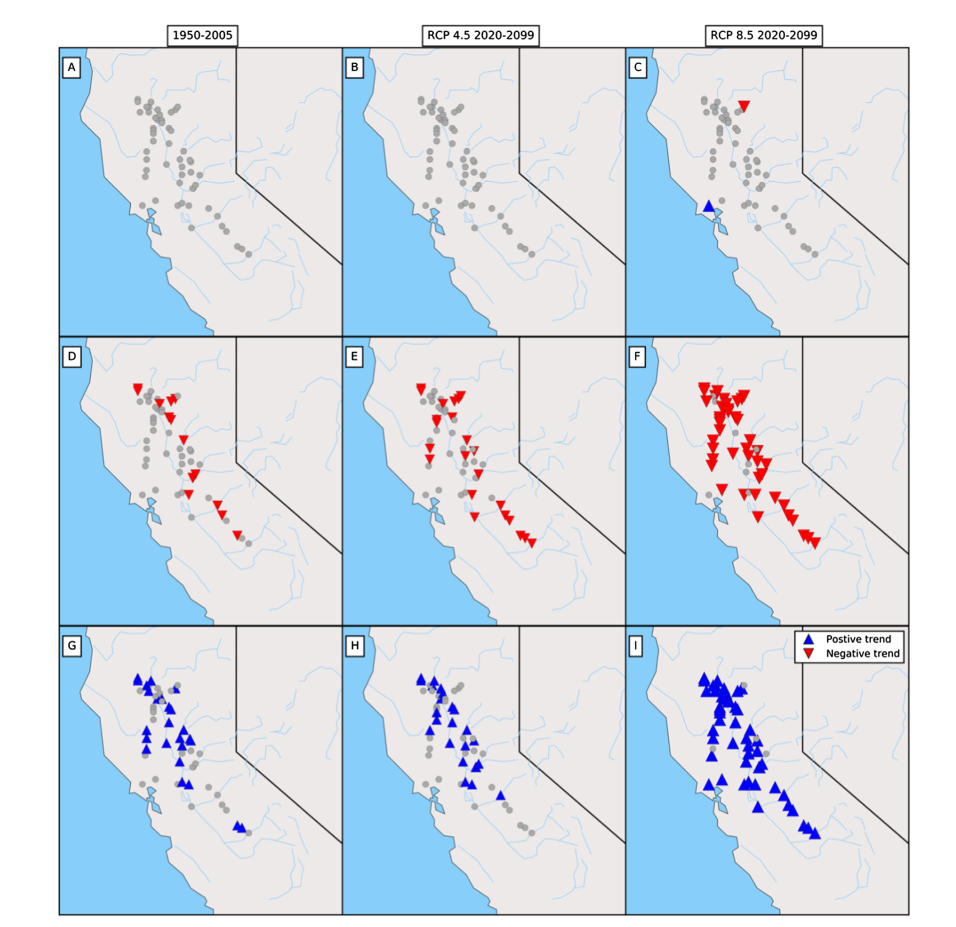
\includegraphics[width=0.5\textwidth]{stream_flow_cali}
    \captionof{figure}{Future Streamflow trends}
    \label{fig:streamflow}
}\end{minipage}

\par In \textit{Figure 1}, notice the minimum streamflow values (red-down arrows) in panels (D-F). In D-panel, there are more reports on negative trends occurring in streamflow values from 1950-2005 which means that inland streams are displaying a decreasing mean during the dry seasons and in G-panel and during the wet season, there is increase in the mean streamflow value. The increase in mean during the wet-season promotes more floods and decrease in mean during dry-season promotes more droughts \autocite{mallakpour_2018}. Although the trends are minor from 1950-2005, the cumulative distribution for future trends highlight a negative trend. Cumulative distribution is likelihood or probability for non-discrete to occur at any given point ranging from one to zero, usually referred to as a random variable. In the current context, the random variable is streamflow discharge (\si{\cubic\meter\per\second}) \autocite{cdf_def}.\\

%Fig. 2
{\begin{minipage}[c]{\textwidth}
\centering   
    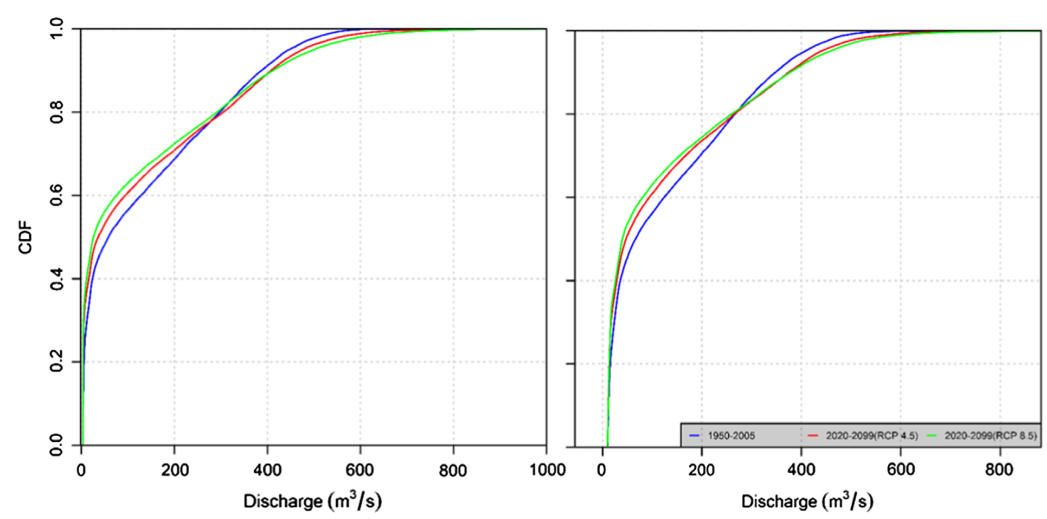
\includegraphics[width=0.75\textwidth]{cdf_streamflow}
    \captionof{figure}{Empirical Cumulative Distribution Functions (ECDFs) of streamflow in the baseline (blue line) and projection periods (red line RCP 4.5 and green line RCP 8.5)}
    \label{fig:cdf}
\end{minipage}}
\vspace{-7pt}

\par \textit{Figure 2} highlights cumulative trend which displays the cumulative distribution of three dataset -- (1) 1950-2005 (2) RCP 4.5 2020-2099 (3) RCP 8.5 2020-2099. The left panel is Oroville Lake in California and the right panel is Shasta Lake. Notice the blue line's distribution is greater than the two project trends from RCP 4.5 and RCP 8.5. RCP 4.5 is a model of future streamflow using using a bias-corrected projection and RCP 8.5 uses data derived from global climate model (GCM) to simulate future streamflows. GCM data is known to have systematic error (biases) due to limited GIS spatial resolution which is why one (RCP 4.5) of the two future projections uses a bias correction projection to account for theses errors (biases).\\

%Fig. 3
\begin{minipage}[c]{\textwidth}{
\centering   
    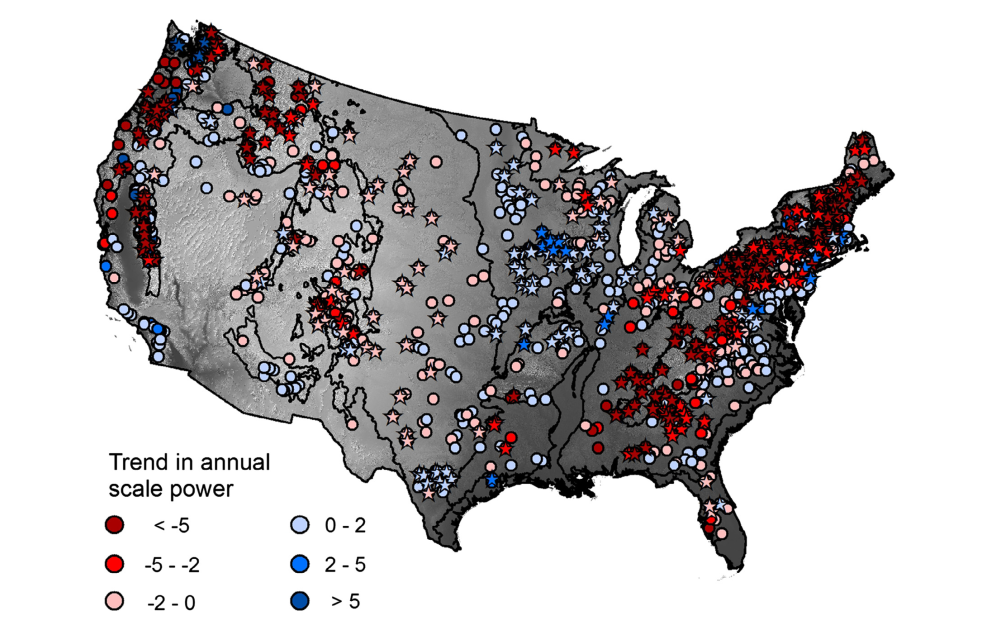
\includegraphics[width=0.8\textwidth]{conus_trend}
    \captionof{figure}{The estimated magnitude of trends in annual scale wavelet power of monthly streamflow from 1940 to 2009. Marker locations indicate watershed centroids. Marker colors in shades of red indicate watersheds with decreasing trends and marker colors in shades of blue indicate watersheds with increasing trends.}
    \label{fig:cdf}
}\end{minipage}
\smallskip

\par But how does climate change affect streamflow variability? From \textcite{rice_2016} study, atmospheric variables may be potential drivers in streamflow variability. \textcite{rice_2016} results suggest that human activities may magnify or amplify the expression of changes. $P_\textit{mean}$ (Precipitation) and $DI_\textit{mean}$ (Dryness index) which were the important atmospheric variables that acted as drivers. There were more variables being used by United State Geological Survey (USGS) but watershed climatology, for instance was too varied amongst CONUS watersheds. \textit{Figure 3} models streamflow trends across the CONUS \autocite{rice_2016}.
\medskip

\section{Literature Review} Water and climate change are quickly becoming global and political issues and many of these issues relate with national security and human health. Before the 70's, obtaining topological images without the aide of computers was a chore that many scientists did not like to do. Even after receiving images or maps, the accuracy may not or may have been the best because of the decentralized nature of information and standards back then. With better systems for acquiring maps, like the Internet, has boosted research interests into hydrological systems in order to understand water and climate change issues \autocite{bras_1999}. In \textcite{bras_1999} article, he believes the studies of groundwater hydrology led scientists interests into the impact of understanding the variables that affect certain properties with hydrology, particularly flow and transport.

\section{Conclusion} The results from \textcite{rice_2016} conclude that climate change does and has affected streamflow in CONUS which serve as sources for freshwater,


\printbibliography

\end{document}
